\chapter{ROOT-based offline event display}
\label{chap:five}

\begin{figure}[htbp]
\centering
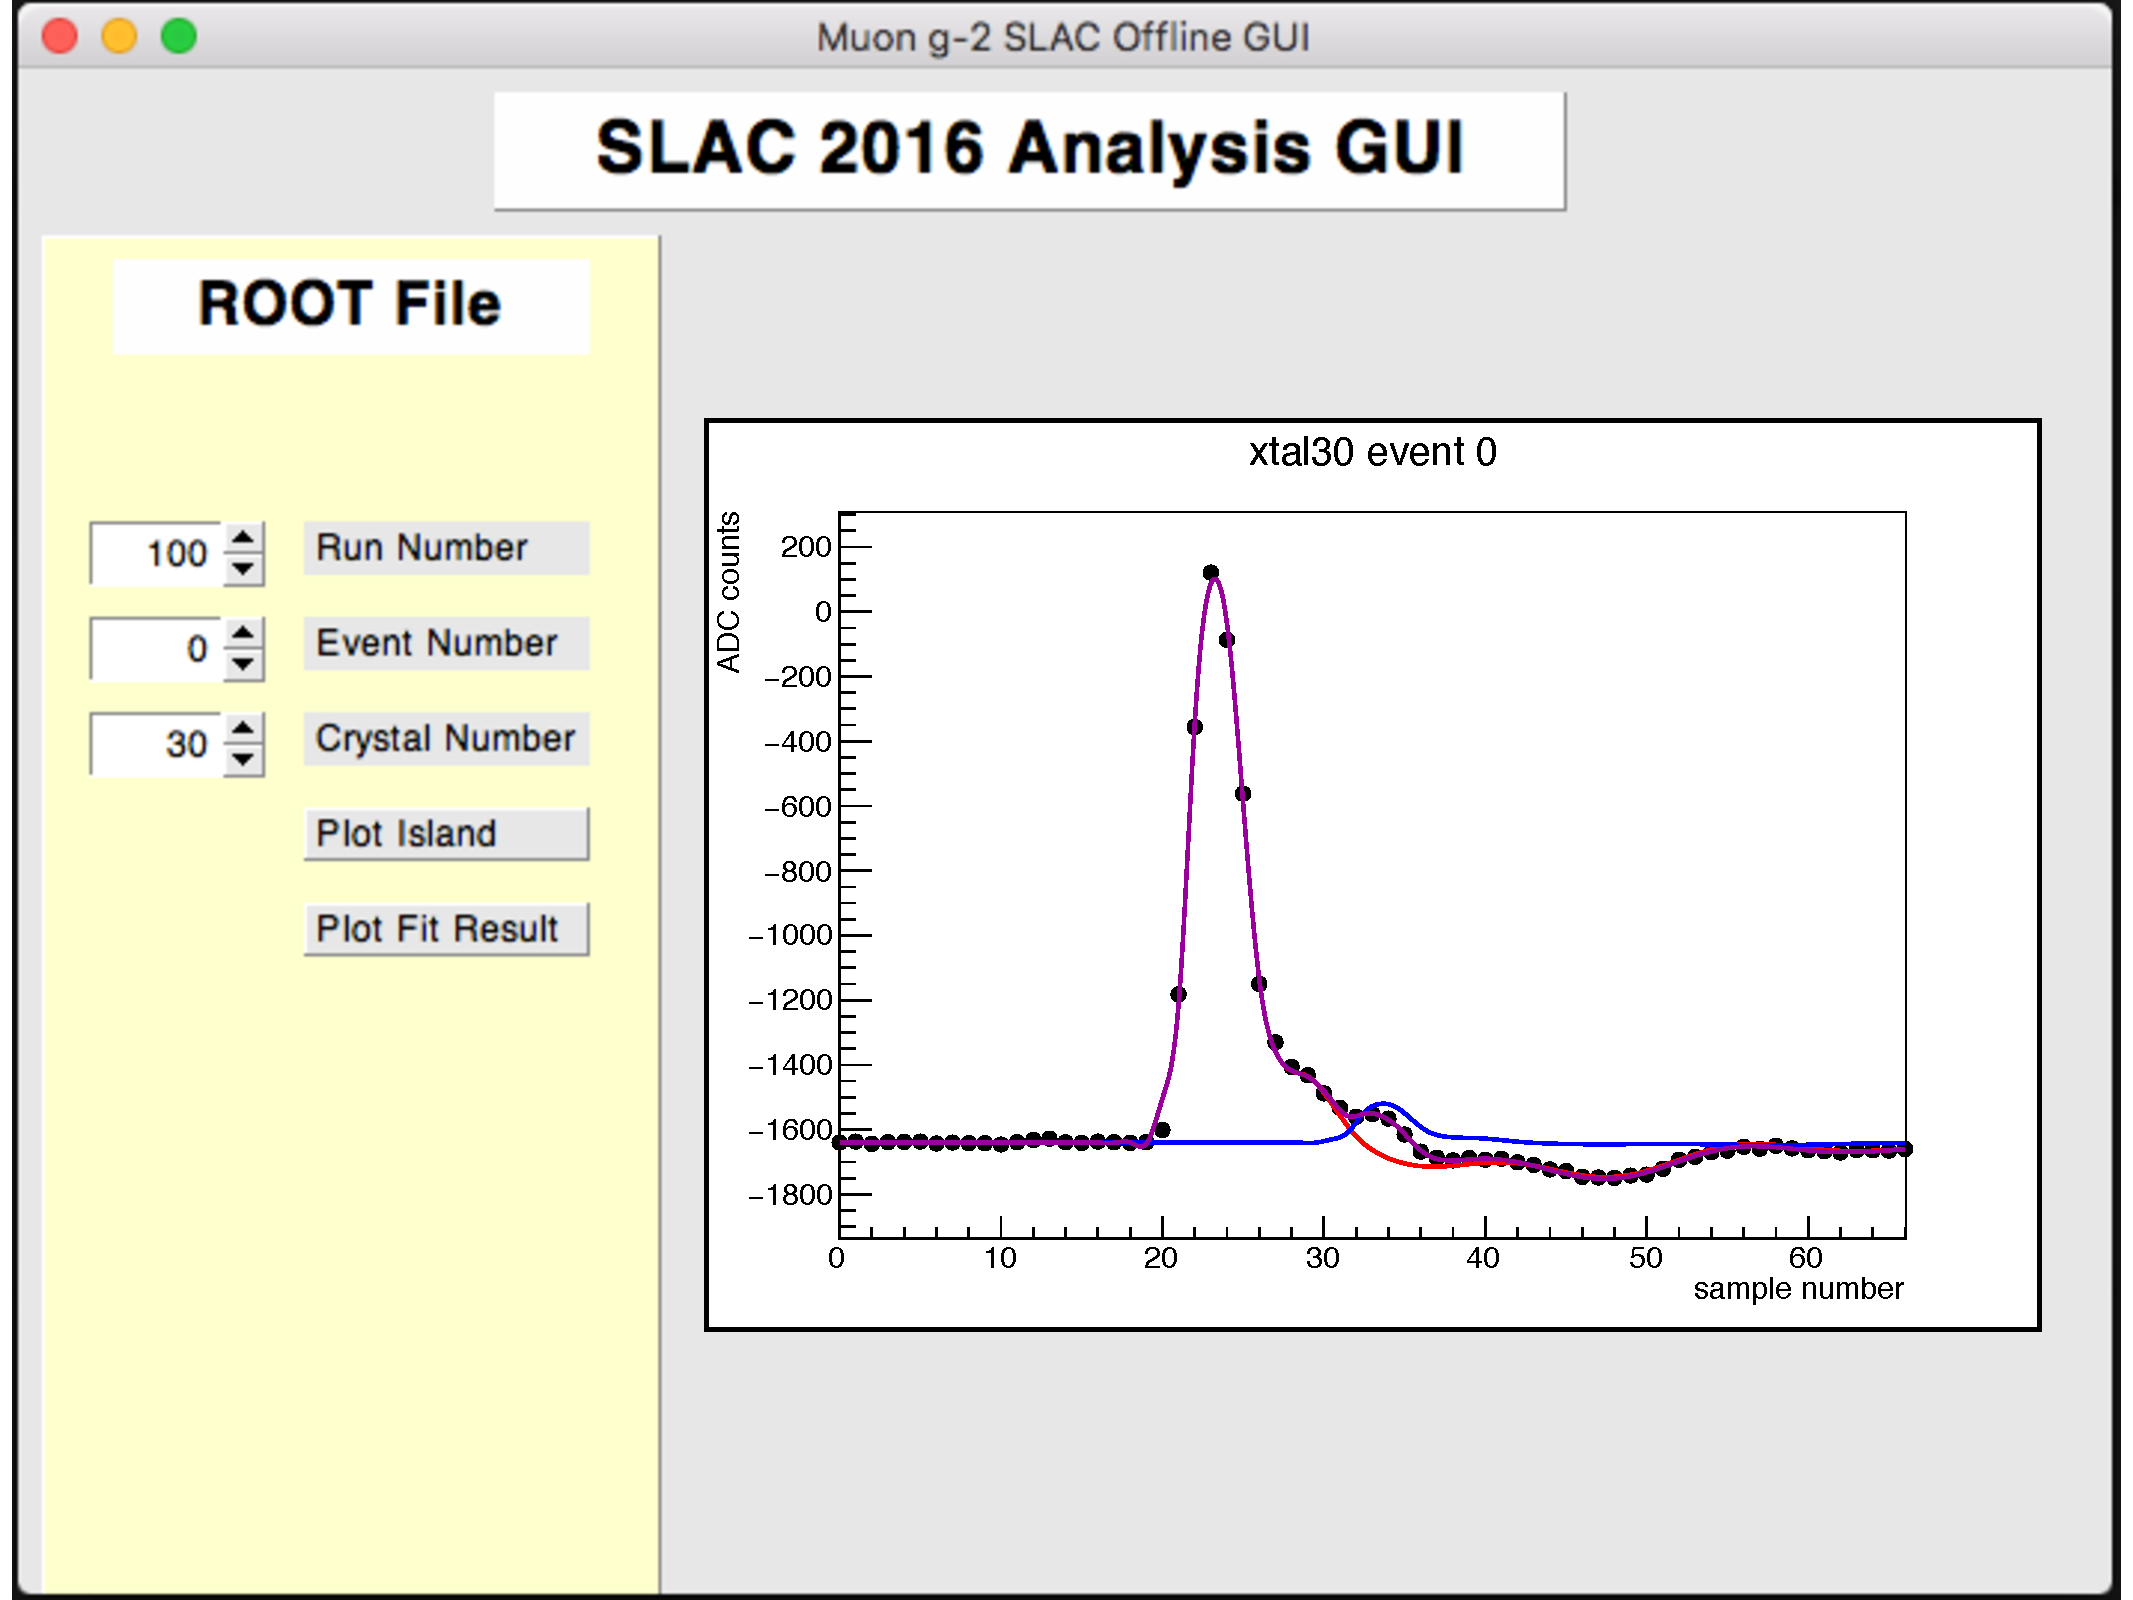
\includegraphics[width=0.6\textwidth]{pics/SLAC2016_Analysis_GUI}
\caption{SLAC Offline analysis GUI. This is a very preminary prototype.}\label{fig:GUI}
\end{figure}

A ROOT-based offline event display is also developed to increase the user friendliness of the data analysis. As shown in Figure~\ref{fig:GUI}, this GUI interface allows the user to inspect the fit results of the template fit algorithm by overlaying it with the island samples. Currently only an executable \verb+eventViewer+ is being developed instead of the full GUI interface.  More functionality will be added in the coming days. 

To compile the code, you need to have ROOT installed and the path set properly.
%
\begin{Verbatim}[frame=single]
cd Offline_GUI/
make
\end{Verbatim}

To execute the code,
%
\begin{Verbatim}[frame=single]
./eventViewer ROOTFILE
\end{Verbatim}
